\section*{Introduction}
Dans ce chapitre, nous présenterons quelques travaux antérieurs dans le domaine
de la transcription automatique de la musique et de la batterie afin de situer
notre démarche. Nous aborderons ensuite le passage crucial du monophonique au
polyphonique dans la transcription. Puis nous décrirons les deux grandes
parties de la TAM de bout en bout allant de l’audio vers l’écriture d’une
partition en passant par le format MIDI. Enfin, nous ferons un point sur les
approches linéaires et hiérarchiques afin de trouver un choix pertinent et
équilibré à favoriser.

\section{Du monophonique vers le polyphonique}
Les premiers travaux en transcription ont été faits sur l’identification des
instruments monophoniques\footnote{Instruments produisant une note à la fois,
ou plusieurs notes de même durée en cas de monophonie par accord (flûte,
clarinette, sax, hautbois, basson, trombone, trompette, cor, etc…)}
\cite{future_directions}. Actuellement, le problème de l’estimation automatique
de la hauteur des signaux monophoniques peut être considéré comme résolu, mais
dans la plupart des contextes musicaux, les instruments sont polyphoniques
\footnote{guitare, piano, basse, violon, alto, violoncelle, contrebasse,
glockenspiel, marimba, etc…}. L’estimation de hauteurs multiples est le
problème central de la création d’un système de transcription de musique
polyphonique. Tout signal audio musical peut être composé de plusieurs signaux,
ceux-ci pouvant provenir de plusieurs instruments, ou d’un instrument dit
polyphonique. Séparer, à partir du signal, les différentes sources audio (ou
voix) afin de les représenter individuellement est une tâche difficile. La
batterie, composée de plusieurs instruments (caisse claire, grosse caisse,
cymbales, toms, etc…), est un cas typique d’intrument polyphonique pour lequel
ce défi est majeur .

Les performances des systèmes actuels ne sont pas encore suffisantes pour
permettre la création d’un système automatisé capable de transcrire de la
musique polyphonique sans restrictions sur le degré de polyphonie ou le type
d’instrument. Cette question reste donc encore ouverte.

\section{De l’enregistrement audio vers le format MIDI}
\label{audio_to_midi}
Jusqu’à aujourd’hui, les recherches se sont majoritairement concentrées sur le
traitement de signaux audio vers la génération de contenus MIDI non-quantifiés
(qui constituent la représentation symbolique d’une performance musicale)
\cite{AMT_for_2_Instru}. Cette tâche englobe plusieurs sous-tâches dont
la séparation des sources audio, la détection multi-\textit{pitchs} \footnote{
    La détection multi-\textit{pitchs} est la
détection des hauteurs simultanées pour les instruments polyphoniques. Il peut
s’agir de notes d’un même instrument ou de plusieurs instruments différents.}
et la détection des \textit{onsets} et des \textit{offsets}.

En transcription automatique de la batterie \cite{Review_ADT}, plusieurs
stratégies de répartition pré/post-\textit{processing} sont possibles pour la
détection multi-\textit{pitchs}. La détection peut être entamée dès le
pré-\textit{processing}, en supprimant les \textit{features}\footnote{
Features~ : caractéristiques individuelles mesurables d’un phénomène dans le
domaine de l’apprentissage automatique et de la reconnaissance des formes.}
non-pertinentes pendant la séparation des sources afin d’obtenir une meilleure
détection des instruments de la batterie, par exemple en supprimant la
structure harmonique pour atténuer l’influence des instruments à hauteurs sur
la détection grosse caisse et caisse claire. Mais certaines études montrent que
la suppression des instruments à hauteurs peut avoir des effets néfastes sur
les performances de la transcription de batterie. En outre, les systèmes de TAB
basés sur des réseaux de neurones récurrents ou sur des factorisations
matricielles font la séparation des sources pendant l’optimisation, ce qui
réduit la nécessité de la faire pendant le pré-processing. Pour la
reconnaissance des instruments de la batterie, une autre approche possible est
d’utiliser un modèle probabiliste pour classifier les différents sons de la
batterie \cite{Eronen}. L’approche AdaMa \cite{adama_1}, qui commence par une
estimation initiale des sons de la batterie en les raffinant itérativement, est
une autre approche de la même catégorie.

Ces méthodes visent toutes la génération d’un contenu MIDI non-quantifié qui
est la représentation symbolique d’une performance musicale.

\section{Du format MIDI vers une partition}
Les approches mentionnées en section \ref{audio_to_midi} produisent en sortie
un fichier MIDI non-quantifié, qui est un format encore très éloigné d’une
partition musicale. Un premier problème concerne les \textit{timings} (dates et durées
d’événements) qui doivent être alignés sur des positions temporelles
correspondant à des valeurs exprimables avec la notation musicale (voir la
différence entre contenu MIDI et musique écrite en section 1.4). On parle de
quantification rhythmique.

Nakamura \textit{et al.} 2016 présentent une approche de quantification rythmique avec
un modèle probabiliste qui prend en entrée un fichier MIDI non quantifié
et fourni en sortie un fichier MIDI quantifié. Shibata \textit{et al.} 2021 \cite{shibata} étendent
ensuite l’approche à une transcription d’enregistrement audio vers un fichier
MIDI quantifié. Ce dernier format, linéaire, ne correspond toutefois pas encore
à une partition structurée,  avec groupement rythmique hérarchique (voir la
section 1.4). Dans ces travaux, la structuration des données en partition est
déléguée à un éditeur de partitions (MuseScore), avec des résultats assez
inégaux.

Seuls quelques travaux récents s’intéressent de près à la création d’outils
permettant la génération de partition. Le problème de la conversion d’une
séquence d’évènements musicaux symboliques en une partition musicale structurée
est traité notamment dans \cite{foscarin}. Ce travail, qui vise à
résoudre de manière conjointe la quantification rythmique et la production de
partitions structurées, s’appuie tout au long du processus sur des grammaires
génératives qui fournissent un modèle hiérarchique — langage \textit{a priori} des
partitions.

Les expériences parviennent à des résultats prometteurs, mais il faut relever qu’elles
ont été menées avec un ensemble de données composé d’extraits monophoniques. Il
reste donc à traiter le passage au polyphonique, qui nécessite de traiter le
problème supplémentaire de la séparation de voix, en le couplant avec la
quantification du rythme. L’approche de \cite{foscarin} est fondée sur la
conviction que la complexité de la structure musicale dépasse les modèles
linéaires.

\section{De l’approche linéaire vers l’approche hiérarchique}

\begin{figure}[h]
	\centering
	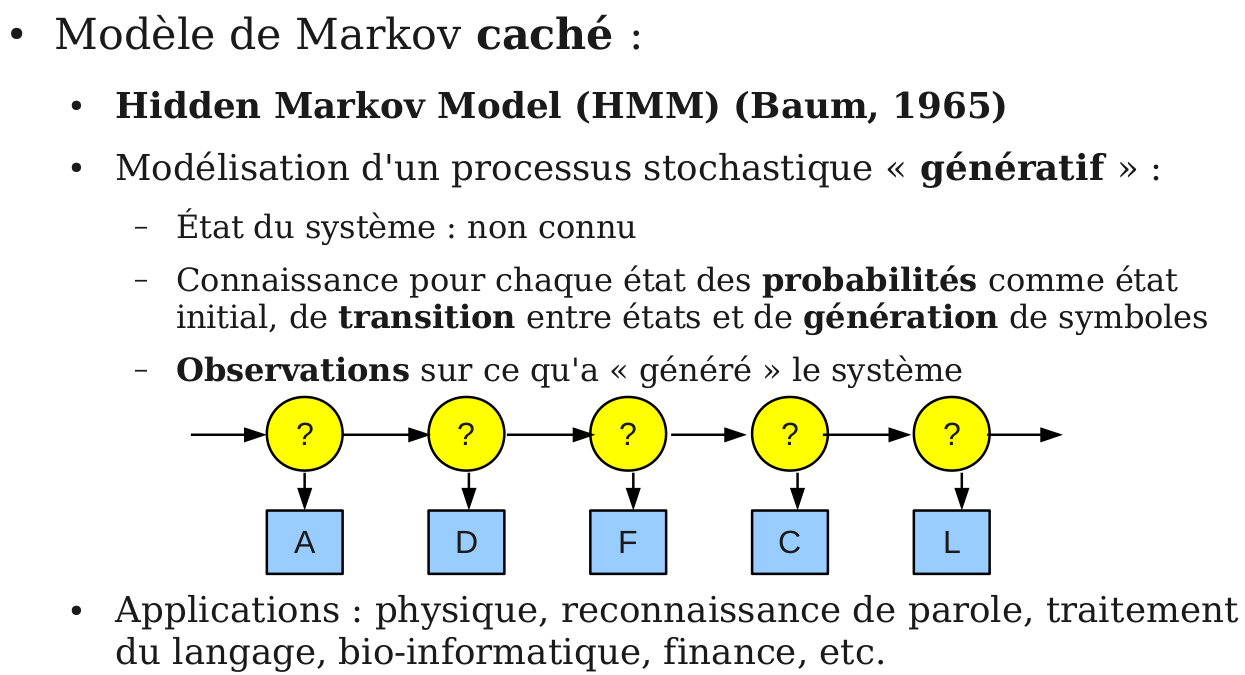
\includegraphics[height=50mm, width=90mm]{
    z_images/2_etat_de_l_art/0_hmm.png}
	\caption[Le modèle de Markov caché]{Le modèle de Markov caché\footnotemark}
    \label{mmc}
\end{figure}

La figure \ref{mmc} montre un exemple de modèle linéaire~ : le modèle de Markov
caché (MMC). Ce type de modèle traite les évènements localement les uns après les
autres. La figure mentionne entre autres que les MMC sont utilisés en
reconnaissance de la parole. Il est intéressant de relever que la
représentation écrite de la parole est linéaire puisque les évènements sont lus
les uns après les autres avant que l’on puisse percevoir la structure d’une
idée. Ce dernier point constitue une différence notable entre l’écriture de la
parole et la notation musicale puisque cette dernière est explicitement
structurée (voir le tableau \ref{spToTxt_vs_TAM}).

Plusieurs travaux ont d’abord privilégié l’approche stochastique. Par exemple,
Shibata \textit{et al.} \cite{shibata} ont utilisé des MMC pour la
reconnaissance des signatures rythmiques. Les auteurs utilisent d’abord deux
réseaux de neurones profonds, l’un pour la reconnaissance des \textit{pitchs}
et l’autre pour la reconnaissance de la vélocité. Ils construisent ensuite
plusieurs MMC étendus pour la musique polyphonique correspondant à des
signatures rythmiques potentielles afin de trouver la signature la plus
probable. L’évaluation finale des résultats de \cite{shibata} montre
qu’il faut \footnotetext{Source~ : cours de Damien Nouvel \url{
https://damien.nouvels.net/fr/enseignement}} rediriger l’attention vers les
valeurs des notes, la séparation des voix et d’autres éléments délicats de la
partition musicale qui sont significatifs pour son interprétation.

Même si la quantification du rythme se fait le plus souvent localement en
manipulant des données linéaires, par déduction de la probabilité d’une durée à
partir de la durée précédente (par exemple dans un MMC), de nombreux travaux
suggèrent d’aborder le problème plus globalement en utilisant une approche
hiérarchique puisque le langage musical est lui-même structuré.

En effet, l’utilisation d’arbres syntaxiques semble appropriée pour représenter
le langage musical. Une méthodologie simple pour la description et l’affichage
des structures musicales est présentée dans \cite{rythm_tree}. Les arbres de
rythmes y sont évoqués comme permettant une cohésion complète de la notation
musicale traditionnelle avec des notations plus complexes. Jacquemard
\textit{et al.} \cite{jacquemard_1} proposent aussi une représentation
formelle du rythme, inspirée de modèles théoriques antérieurs issus du domaine
des techniques de réécriture appliquées à la déduction automatique et au calcul
symbolique. Ils montrent aussi qu’il est possible d’appliquer des arbres de
rythmes pour le calcul d’équivalences rythmiques dans
\cite{jacquemard_2}. La réécriture d’arbres, dans un contexte de
composition assistée par ordinateur, par exemple, pourrait permettre de
suggérer à un utilisateur diverses notations possibles pour une valeur
rythmique, avec des complexités différentes.

La nécessité d’une approche hiérarchique pour la production automatique de
partition est évoquée dans \cite{foscarin}. 
Les modèles de grammaire qui y sont exposés sont différents des modèles
markoviens linéaires de précédents travaux.

L’analyse de la structure hiérarchique des séquences d’accords par utilisation
de modèles grammaticaux s’est avérée très utile dans les analyses récentes de
l’harmonie du jazz \cite{harasimjazz}. 


\begin{figure}[h]
	\centering
	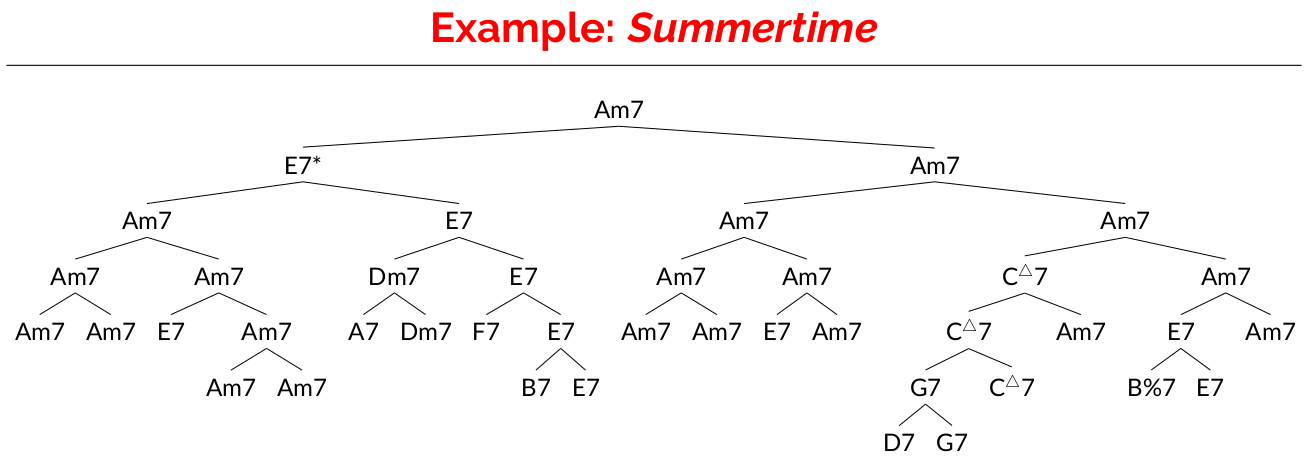
\includegraphics[height=40mm, width=120mm]{
    z_images/2_etat_de_l_art/1_summertime_tree.png}
    \caption{Représentation arborescente d’une grille harmonique
    \protect\cite{harasimjazz}}
    \label{arbre_harmo}
\end{figure}

La figure \ref{arbre_harmo} est une représentation dans un arbre syntaxique de
la structure harmonique du standard de jazz \textit{Summertime}. La racine de l’arbre
est la tonalité du morceau. Entre la racine et les feuilles se trouve la
structure harmonique qui défile en fonction des différentes parties du morceau
et les feuilles représentent les accords joués.

\section*{Conclusion}
La plupart des travaux déjà existants sur la TAB ont été énumérés par Wu
\textit{et al.} \cite{Review_ADT} qui, pour mieux comprendre la pratique des
systèmes de TAB, se concentrent sur les méthodes basées sur la factorisation
matricielle et celles utilisant des réseaux neuronaux récurrents. La majorité
de ces recherches se concentre sur des méthodes de calcul pour la détection
d’événements sonores de batterie à partir de signaux acoustiques ou sur la
séparation entre les évènements sonores de batterie avec ceux des autres
instruments dans un orchestre ou un groupe de musique \cite{2802}, ainsi que
sur l’extraction de caractéristiques de bas niveau telles que le classement des
instruments et le moment de l’apparition du son. Très peu d’entre eux ont
abordé la tâche de générer des partitions de batterie et, même quand le sujet
est abordé, l’\textit{output} final n’est souvent qu’un fichier MIDI
non-quantifié et non une partition écrite.\\

En conclusion, il n’existe pas de formalisation de la notation de la batterie
ni de réelle génération de partition finale, dont les enjeux principaux
seraient~ :
\begin{enumerate}
    \item le passage du monophonique au polyphonique, comprenant la distinction
        entre les sons simultanés et les appogiatures\footnote{Les appogiatures
        sont des ornements qui se placent devant une note principale et qui est
    jouée presque simultanément.}~ ;
    \item les choix d’écritures spécifiques à la batterie concernant la
        séparation des voix et les continuations.
\end{enumerate}
